\chapter{Modeling Attempts}

\section{Simple Model from Scratch}
\subsection{Simple ODE Model}
Here, we develop a model that keeps track of the following variables
\begin{quote}
	$n(t)$= density of tip cells in area of interest, (number per unit area).
	
	$\rho(t)$ = density of blood vessels (length per unit area).
	
	$c(t)$ = concentration of drug delivered to region by blood vessels (nano mole per unit area).
\end{quote}
An updating list of model parameters:
\begin{itemize}
	\item $v$ [length/time]: The rate at which the tip cells move and extends the blood vessels.
	\item $\delta_v$ [1/time]: The rate at which the vascular structure gets degraded.
	\item $\lambda_s$ [1/time]: Tip cell division rate (splitting rate).
	\item $\lambda_b$ [1/time/length]: Tip cell emerging rate from stalk cells.
	\item $\delta_t$ [1/time]: Tip cell death/deactivation rate.
	\item $\kappa$ [area/length/time]: Re-connection of tip cells to the other capillaries to form loops.  
	\item $\mu$ [1/time]: Permeability of the capillary to the drug. 
	\item $\sigma$ [area/length]: The coverage of the blood vessels in the region.
\end{itemize}
And a list input functions
\begin{itemize}
	\item $f(t)$: [nmol/length]: The amount of drug inside the capillary.
\end{itemize}




\subsection*{Studying dynamics of vessel formation}
\[ \frac{d\rho}{dt} = ??. \]
The active tip cells extend the vascular structure as they move. Assuming the tip cells move at rate $v$, then 
\[ \frac{d \rho}{dt} = vn+ ??. \]
Also, assuming the vascular structure degrades with rate $\delta$ [per unit time], we can add the degradation term 
\[ \boxed{\frac{d\rho}{dt} = vn - \delta_v \rho} . \]



\subsubsection*{Studying the Dynamics of Tip Cells}
Things important in the dynamics of the tip cells
\begin{itemize}
	\item Generation of the tip cells: There are at least two ways for new tip cell generation listed as follows:
	\begin{enumerate}[(i)]
		\item Splitting mechanics: When the tip cells splits new vascular stem gets two heads. This should be proportional to the density of tip cells. The parameter $\lambda_s$ [per unit time] reflects this mechanism.
		\item Branching: New tip cells can form out the the endothelial stalk cells. This process should be proportional to the density of blood vessels. The parameter $\lambda_b$ [per unit time per unit length] reflects this mechanism
	\end{enumerate}
	\item Loss of tip cells
	\begin{enumerate}[(i)]
		\item Death of the tip cells or getting deactivated: Reflected by the parameter $\delta_t$
		\item Joining the other branches of vascular network: When a tip cell reconnects another capillary branch, then they disappear. The parameter $\kappa$ is for this mechanism. Note that the re-connection term is proportional to both number of tips cells, as well as the density of blood vessels. Thus the units of $\kappa$ should be [area/length/time]. 
	\end{enumerate}
	\item The movement of tip cells and formation of new vascular networks along the way.
\end{itemize}

\[ \boxed{\frac{dn}{dt} = (\lambda_s - \delta_t) n + \lambda_b \rho - \kappa n \rho}.  \]

\subsubsection*{Nondimensionalization}
In order the analyze the model more easily, we nondimensionalize the system with the following change of variable
\[ \rho = R \tilde{\rho}, \qquad n = N \tilde{n}, \qquad t = T \tau. \]
There are many possible choice to choose the scaling factors $R, N, T$. However, we will choose them in a way that they are always positive, and the system of ODE becomes as simple as possible. Substituting the change of variable above in the ODE system, we will get
\begin{align*}
	&\frac{d\tilde{\rho}}{d\tau} = \frac{vNT}{R}\tilde{n} - \delta_v T \tilde{\rho},\\
	&\frac{d\tilde{n}}{d\tau} = T(\lambda_s-\delta_t)\tilde{n} + \frac{\lambda_b T R}{N} \tilde{\rho} - T\kappa R \tilde{n}\tilde{\rho}. \tag{\twonotes}
\end{align*}
We choose the following values for $T,N$, and $R$
\[ T = \frac{1}{\delta_v}, \qquad R = \frac{\delta_v}{\kappa}, \qquad N = \frac{\lambda_b}{\kappa}. \]
This is a very suitable moment to pause and check the dimensions if they match (I did it and all of them matches!). With these choices from the coefficients, the system of ODEs will be
\[ \frac{d\tilde{n}}{d \tau} = \frac{\lambda_s - \delta_t}{\delta_v} \tilde{n} + \tilde{\rho} - \tilde{n}\tilde{\rho}, \qquad
\frac{d\tilde{\rho}}{d\tau} = \frac{v\lambda_b}{\delta_v^2}\tilde{n} - \tilde{\rho}. \]
To make the ODEs simpler to work with, we will write $n,\rho$ in place of $\tilde{n}$ and $\tilde{\rho}$, and also we introduce the following parameters
\[ \alpha = \lambda_s - \delta_t, \qquad \beta =\delta_v, \qquad \gamma = v\lambda_b. \tag{$\clubsuit$} \]
Then we can write 
\begin{equation*}
	\boxed{
		\begin{aligned}
			&\dot{n} = \frac{\alpha}{\beta}n + \rho - n\rho, \\
			&\dot{\rho} = \frac{\gamma}{\beta^2}n -\rho.
		\end{aligned}
	}
	\tag{\smiley}
\end{equation*}

\begin{observation}[Other form of non-dimensionalization]
	After inspecting the non dimensionalization steps, we can see that the parameter $ \kappa $ somehow disappears, and there is no sign of it in the new parameters $ \alpha, \beta, $ and $ \gamma $. I tried another choices for $ R, T, $ and $ N $, but still, I can not have the $ \kappa $ in the new parameters. The steps that I followed are the following.
	\[ T \kappa R = 1, \qquad NvT/R = 1, \qquad \delta_v T = 1. \]
	Then we will have
	\[ T = 1/\delta_v, \qquad R = \delta_v/\kappa, \qquad N = \delta_v^2/(v\kappa). 
	\]
	Thus the system of ODEs will be
	\[ \dot{\rho} = n - \rho, \qquad \dot{n}= \alpha/\beta n - n\rho + \gamma/\beta^2 p, \]
	where
	\[ \alpha = \lambda_s - \delta_t, \qquad \beta=\delta_v, \qquad \gamma = \lambda_b v. \]
	Still, there is not $ \kappa $ in the new parameters. 
\end{observation}

In order to find the equilibrium points, we demand $\dot{n} = 0$ as well as $\dot{\rho} = 0$. This will lead to the following equations
\begin{align*}
	\dot{n} = 0&: \qquad \frac{\alpha}{\beta} n + \rho - n\rho = 0, \\
	\dot{\rho} =0&: \qquad \frac{\gamma}{\beta^2}n - \rho = 0.
\end{align*}
After some algebra, it turns out that there are two equilibrium points for this system.
\[ p^0_1 = (0,0), \qquad p^0_2 = (\frac{\alpha\beta}{\gamma} + 1, \frac{\gamma}{\beta^2}+\frac{\alpha}{\beta}) = (\frac{\alpha\beta+\gamma}{\gamma},\frac{\gamma + \alpha\beta}{\beta^2}). \tag{E.1.1} \]
%\begin{strangeObs}
%	Something does not make sense! We know that the variables $n$ and $\rho$ must all be positive, as they are both representing biological values. However, by looking closely at the second component of $p^0_2$, it turns out th at $\gamma - \alpha\beta$ should be positive. In order to have the first component positive as well, then $\gamma$ should be negative, which is not possible. That is because by $(\clubsuit)$ we know that $\gamma>0$. There is at least one solution for this paradox, which is letting $\alpha\beta - \gamma =0$. Then this equilibrium point will be the same as $p^0_1$, showing the fact that the system has only one equilibrium point with biological meaning, which is the origin (not very interesting)!\\
%	However, I am going to ignore this observation for now and proceed with the stability analysis.
%	
%	\label{strangeObs:SimpleODEequiliNegative}
%\end{strangeObs}

In order to analyze the stability of these equilibrium points, we first need to calculate the Jacobian matrix of the ODE system 
\[ DF = \matt{\alpha/\beta-\rho}{1-n}{\gamma/\beta^2}{-1}. \]

\subsubsection{Stability Analysis of $p^0_2$}
By evaluating the Jacobian matrix at the equilibrium point we will have
\[ DF[p^0_2] = \matt{-\gamma/\beta^2}{-\alpha\beta/\gamma}{\gamma/\beta^2}{-1}. \]
The trace and determinant of this matrix is
\[  \Delta = \gamma/\beta^2 + \alpha/\beta, \qquad \sigma=-\gamma/\beta^2 - 1.  \]
By close inspection, it turns out that $\Delta$ is the same as the first component of $p^0_2$, which should be positive. This implies $\Delta > 0$. So the sign of the trace of the Jacobian matrix will determine the stability. From $(\clubsuit)$, $\gamma>0$. Thus $\sigma < 0$. This indicates that the equilibrium point $p_0^2$ is stable equilibrium. Also, note that since $\sigma$ can never transversally become positive from being negative (i.e. passing through $\sigma=0$, transversally), thus we can rule out the existence of any Hopf bifurcation with this particular model.

\begin{observation}[stability of $p^0_2$]
	The Jacobian matrix evaluated at $p^0_2$ has
	\[ \Delta \geq 0, \qquad \sigma < 0. \]
	Thus equilibrium point $p^0_2$ is a hyperbolic sink (when $\delta > 0$). This hyperbolic sink can be of the type stable node (with purely real eigenvalues) or stable focus (with complex valued eigenvalues whose real part is negative). But since these two kind of stability are topologically equivalent, we don't do further analysis to distinguish them at this point.
%	When $\Delta>0$, then we have two imaginary eigenvalues
%	\[ \lambda_1 = \sigma/2+i\sqrt{\Delta}, \qquad \lambda_2 = \sigma/2-i\sqrt{\Delta}. \]
%	where $\sigma$ is always negative. This implies that $p^0_2$ will always be a stable focus and the equilibrium point will be approached in a damping oscillatory way.\\
%	In the special case where $\Delta =0$, we will have $p^0_2=p^0_1$, thus it will inherit the stability of $p_0^1$. 
\end{observation}

\begin{observation}[No sustained oscillations]
	Note that since $\sigma<0$ for all values of the parameters of the model, then there is no chance to observe a Hopf bifurcation, thus ruling out any sustained oscillations in the model.
\end{observation}

\subsubsection{Finding Lyapunov Function}
In attempting to find a Lyapunov function, I thought it might be a good idea to have a different choices for the non-dimensionalization scaling so that I can have control on the nonlinear part $n\rho$. But it seems that there are no possible ways to achieve this. That is because in $(\twonotes)$, we can not make the first term of RHS of $\dot{\tilde{\rho}}$ and the second term of RHS of $\dot{\tilde{n}}$ simultaneously to be 1. Thus there are no choices for the scaling factors to make the coefficient of $\tilde{n}\tilde{\rho}$ to be 1.


\subsubsection{Stability Analysis of $p^0_1$}
The Jacobian matrix evaluated at $p^0_1$ is
\[ DF[p^0_1] = \matt{\alpha/\beta}{1}{\gamma/\beta^2}{-1}. \]
The determinant and the trace will be
\[  \Delta = -\alpha/\beta - \gamma/\beta^2, \qquad \sigma = \alpha/\beta-1. \]
\begin{observation}
	The determinant $\Delta$ is negative the first term of the $p^0_2$. Thus $\Delta\leq0$. When $\Delta<0$, then regardless of value of $\sigma$, $p^0_1$ is a hyperbolic saddle. However, when $\Delta=0$, then $p^0_1$ is non-hyperbolic and further analysis is required to determine the stability.
\end{observation}
The following shows the phase portrait of the system with some values for the parameters.
\begin{figure}[h!]
	\centering
	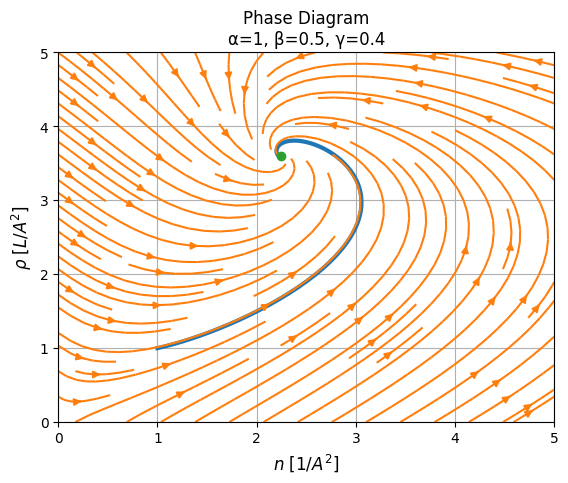
\includegraphics[width=0.5\linewidth]{images/simpleODEModel1PhasePortrait}

	\label{fig:simpleodemodel1phaseportrait}
\end{figure}


Furthermore, the following diagram shows the nullclines and the sign of the vector field at the different regions of the phase portrait.

\FloatBarrier

%\begin{strangeObs}
%	This equilibrium point $p^0_1$ has no choice but to be stable, if we expect the model to represent real biological situation. But our analysis above, reveals that this equilibrium point is in fact a saddle point. However, I can argue that if that the eigenvector with negative eigenvalue for the Jacobian matrix evaluated at $p^0_2$, lies in the first quadrant, then $p^0_2$ will ``look'' stable for the points at the first quadrant. But I am not sure if this is something normal to happen for a biological model.
%\end{strangeObs}


\subsection*{Quantitative analysis with nullclines}
Drawing the phase portrait and including the nullclines helps in understanding the quantitative effect of change in parameters (which causes by the drug-vessel interaction). To draw the nullclines, we require
\[ \vectt{\dot{n}}{\dot{\rho}} = \vectt{f_1(n,\rho)}{f_2(n,\rho)} = \vectt{\frac{\alpha}{\beta}n + \rho - n\rho}{\frac{\gamma}{\beta^2}n - \rho} = \vectt{0}{0}. \]
After a little bit of algebra, we get
\begin{align*}
	\dot{n} = 0:& \qquad \rho = \frac{\alpha}{\beta}\cdot \frac{n}{n-1} \quad (n\neq 1),\\
	\dot{\rho} = 0:& \qquad \rho = \frac{\gamma}{\beta^2}n.
\end{align*}
\begin{observation}
	The reason that we get the restriction $n\neq 1$ for the $\dot{n} = 0$ nullcline is the following. From (E.1.1) we know that $f_1(p^0_2)=0$. Thus we can use the implicit function theorem to get a continuous branch of equilibria near $p_2^0$ in the form of $\rho = \hat{\rho}(n)$ where $\hat{\rho}$ is a continuously differentiable function, where $\rho^* = \hat{\rho}(n^*)$ (note $p^0_2 = (n^*, \rho^*)$), and $f_1(n,\hat{\rho}(n)) = 0$ for some open neighborhood containing $p_2^0$. However, we can use this implicit function argument only when $\partial_\rho f_1 \neq 0$, which implies $n\neq 1$.\\
	Also, it is interesting to note that $n=1$ is equivalent to $\alpha=0$. This can be observed from (E.1.1). The consequences of this are summarized in the following observation boxes.
\end{observation}

We will have two cases of the phase portrait as shown in the figure below. Note that the stability of the equilibrium point $p_2^0$ will still remain the same as the value of $\alpha$ passes $\alpha=0$ transversally. The results of this section is summarized in the observation box below.
\begin{figure}[h!]
	\centering
	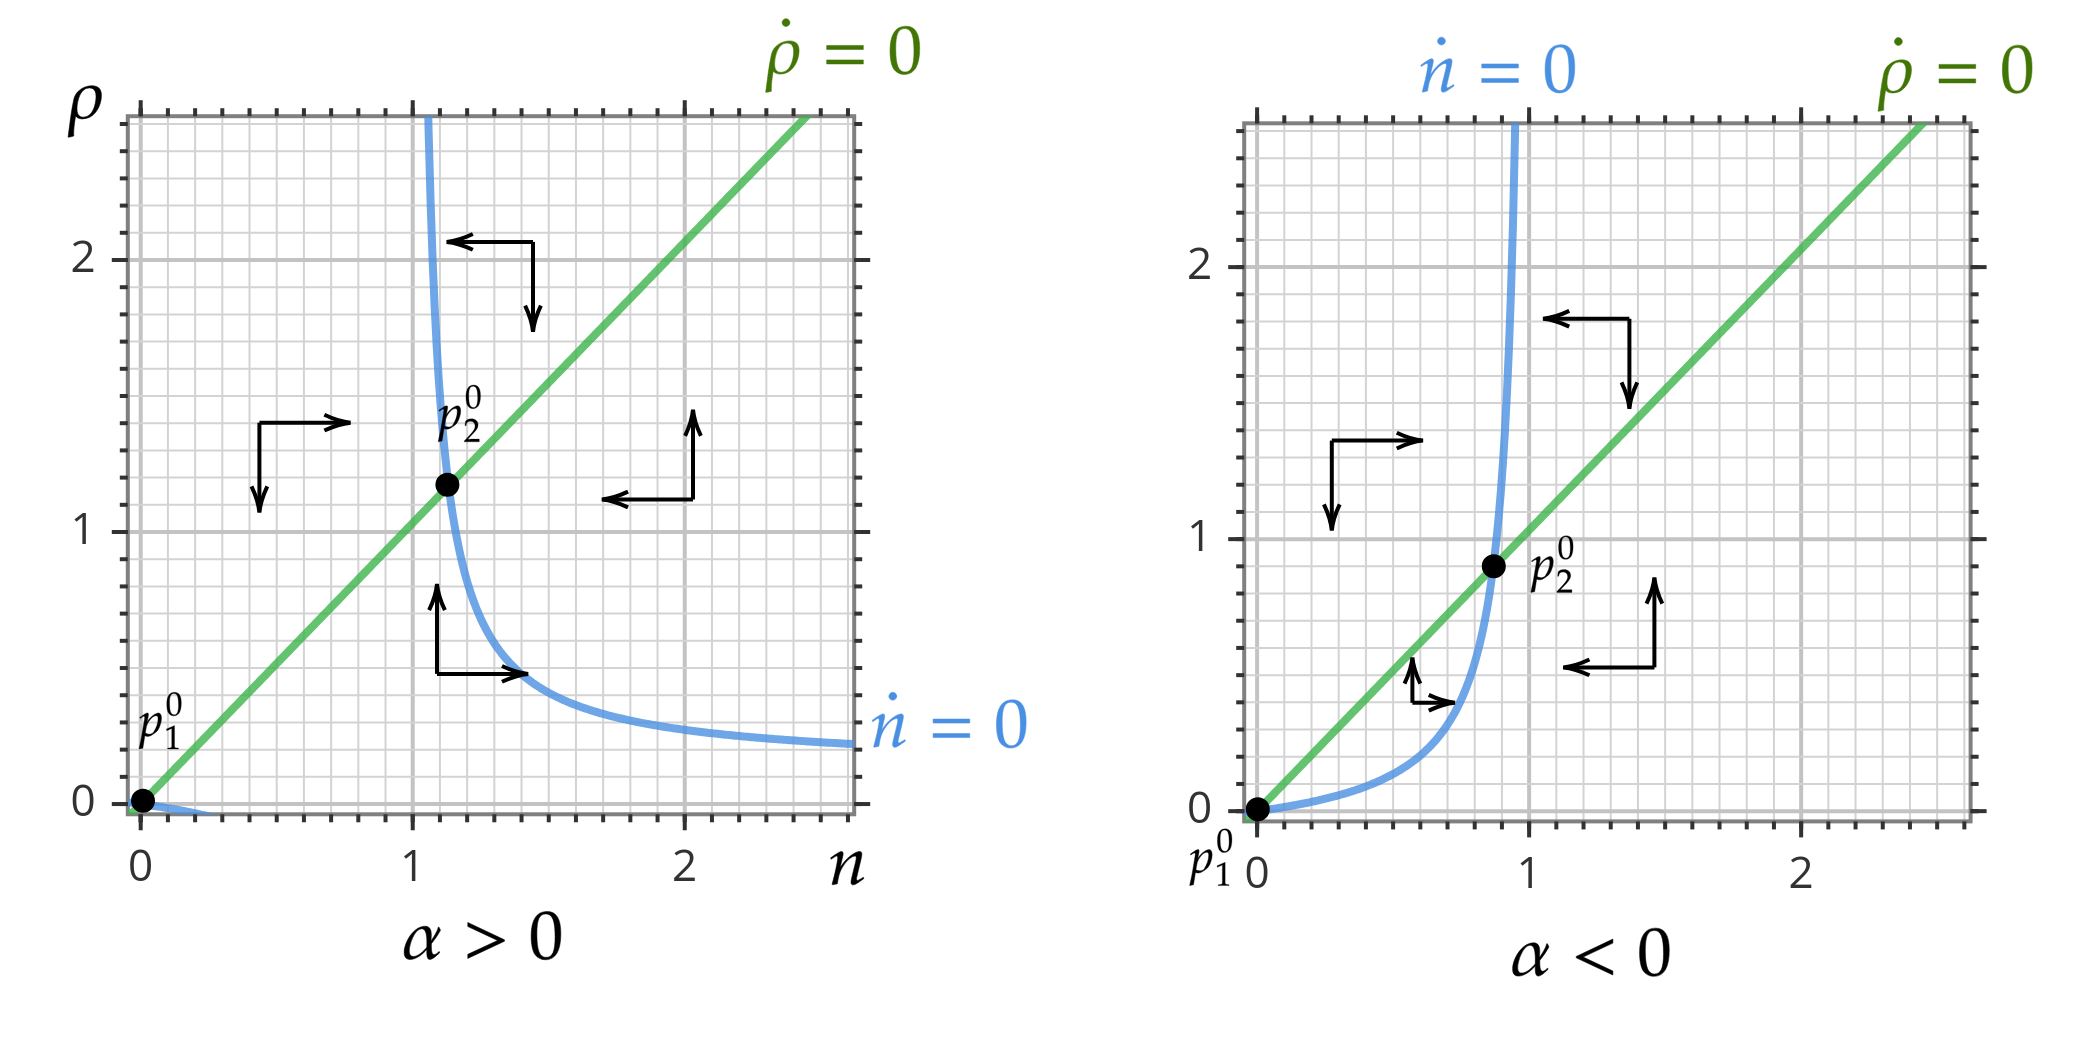
\includegraphics[width=\linewidth]{images/nullClines_positiveNegative.png} % first image
\end{figure}

\FloatBarrier

\begin{observation}[Two different phase portraits]
	As the parameter $\alpha$ passes through $\alpha_0 = 0$ transversally, we get two phase portraits that are not topologically equivalent (the results are shown in the figure above). Because of this, depending on the sign of $\alpha$, we will observe totally different behaviours from the system as we change the parameter values. \\
	I \textbf{emphasis} that in both of these phase portraits, the stability of both equilibria remains the same.
\end{observation}

\begin{observation}[Biological meaning of $\alpha$]
	From $(\clubsuit)$ we see that $\alpha = \lambda_s - \delta_t$, where $\lambda_s$ is the tip cell division rate (which leads to vascular splitting), and $\delta_t$ is the death rate of the tip cells. Thus $\alpha >0$ translates to larger division rate compared to the death rate for tip cells, and $\alpha<0$ is the opposite.
\end{observation}





\subsection*{Quantitative study of Effect of Changing the Parameters}
This section will lay the foundations for studying the drug-vessel interaction and how that affects the system.
\subsubsection*{Effect of $\alpha$} 
Regardless of the sign of $\alpha$ (i.e. being in either of phase portraits) increasing the value of alpha will move the $p^0_2$ higher. This observation is summarized in the following figure.
\begin{figure}[h!]
	\centering
	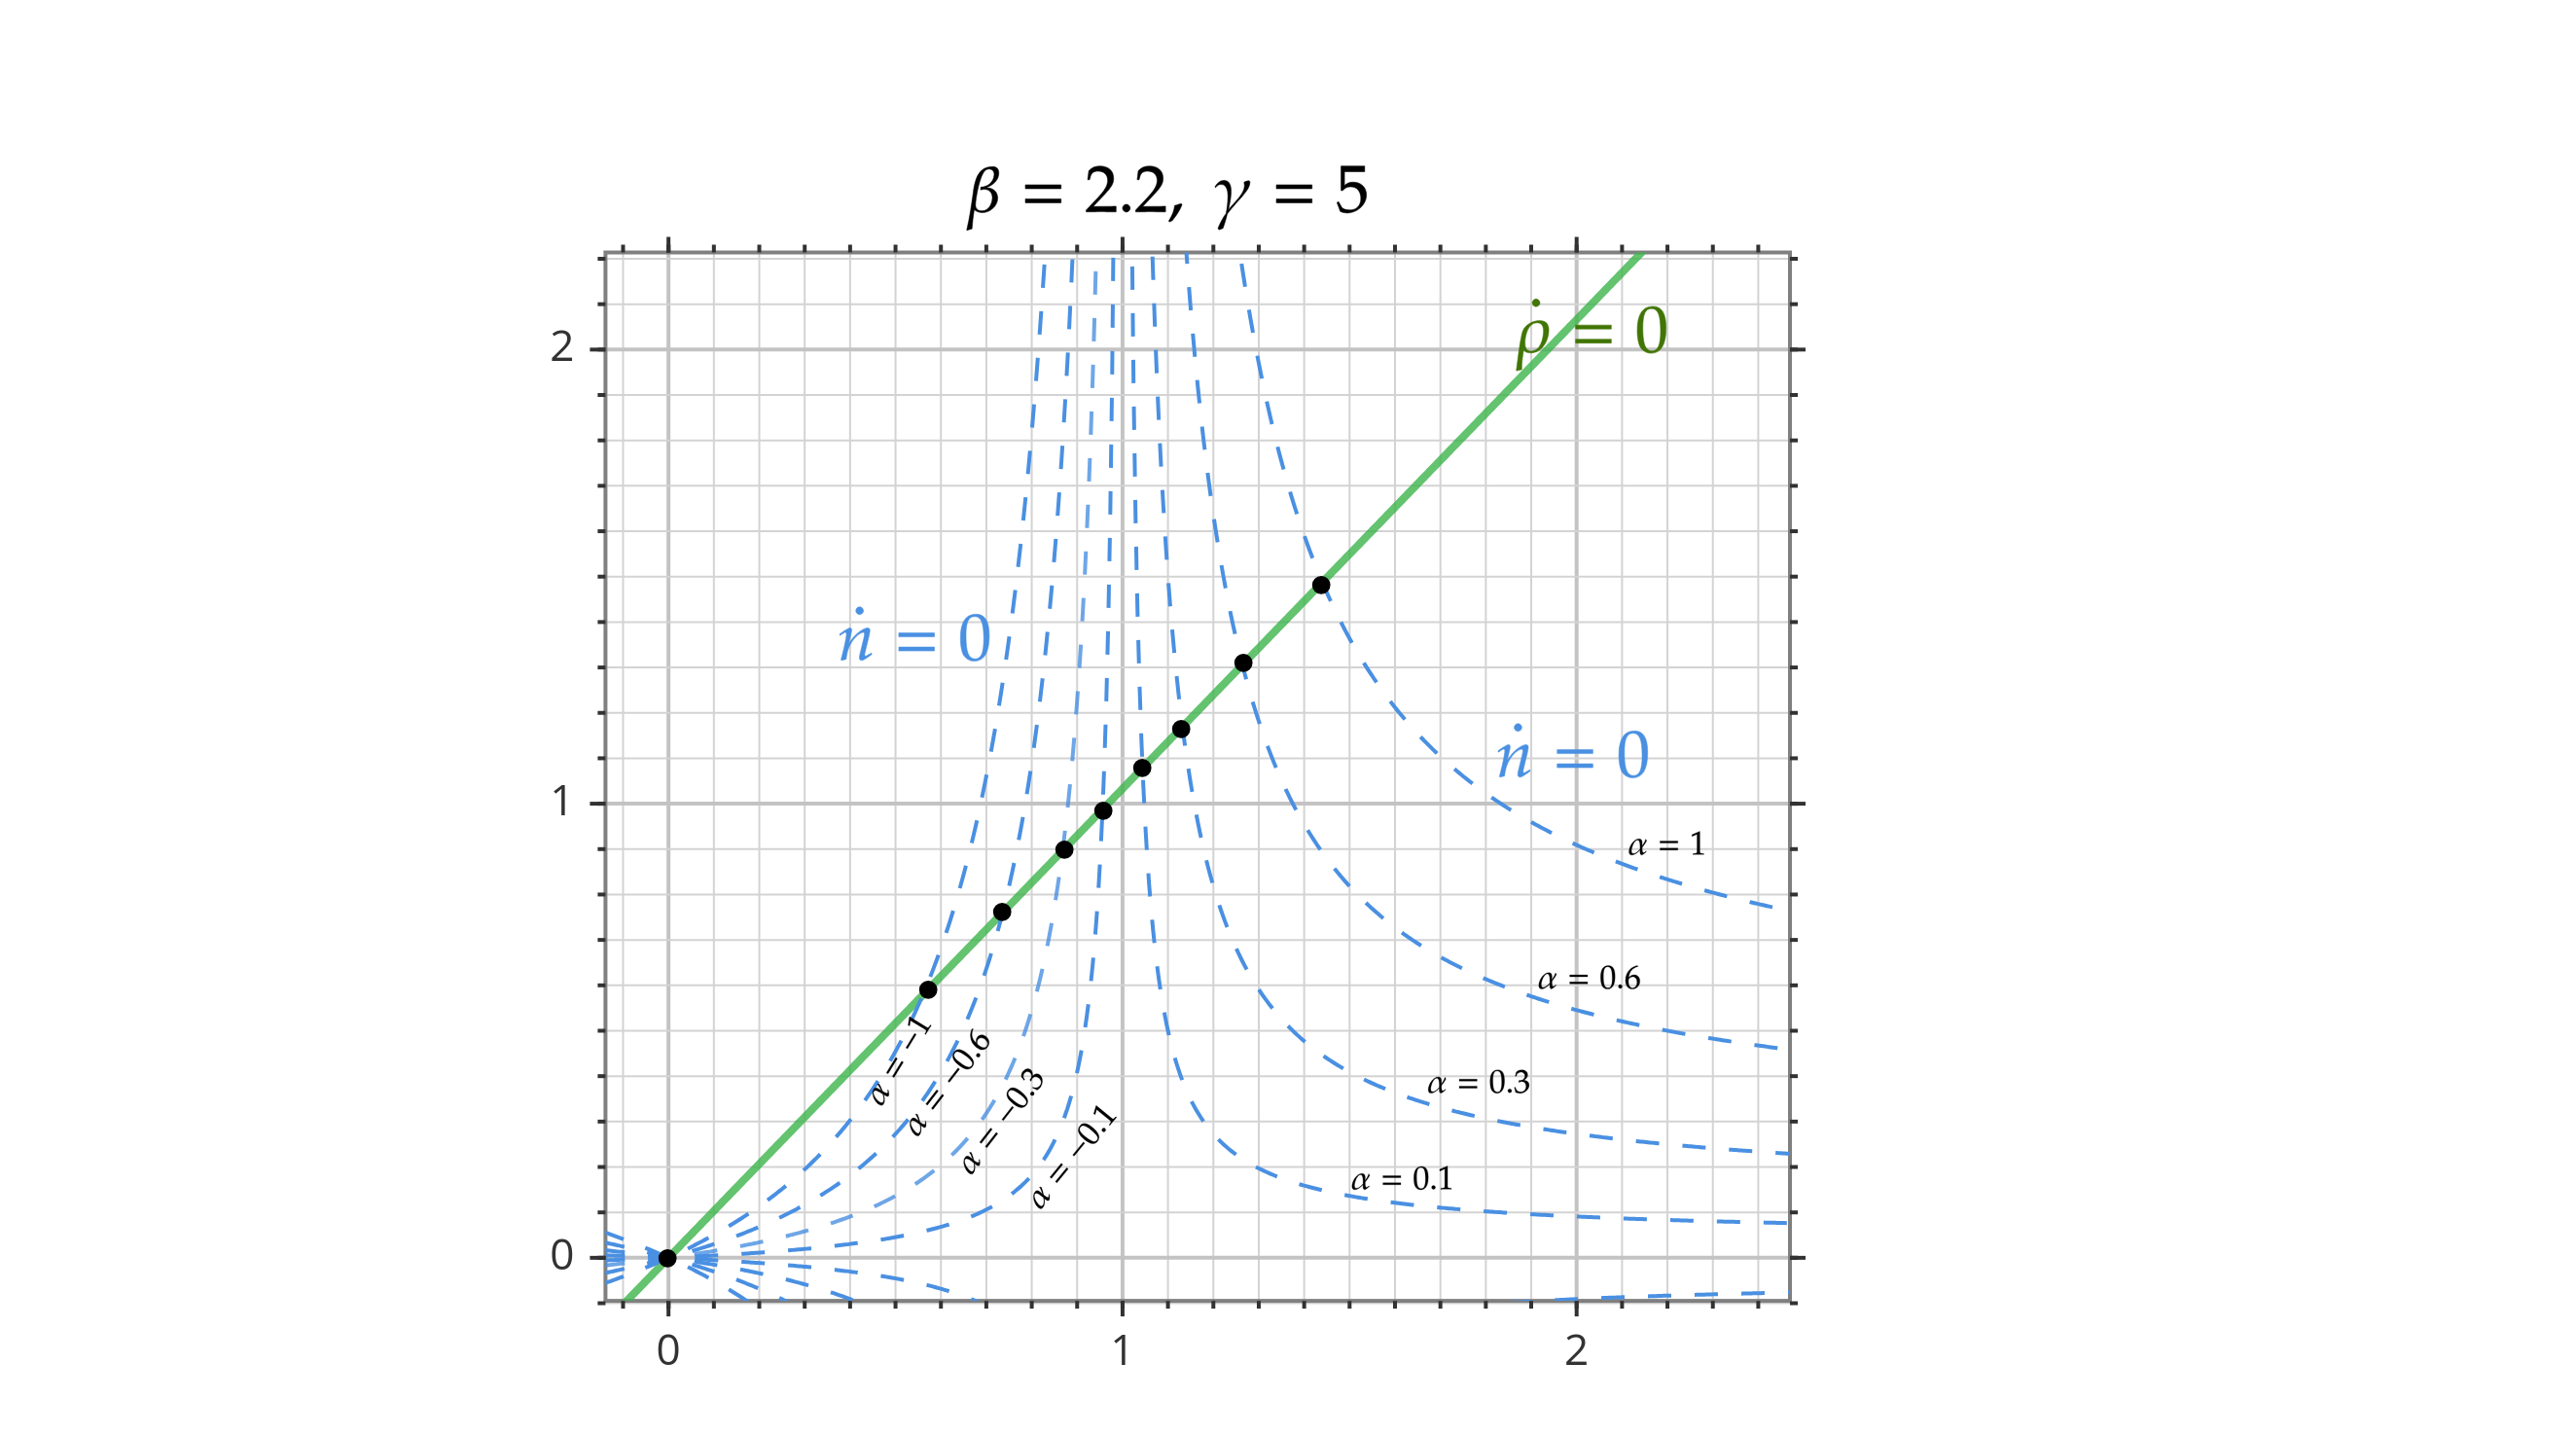
\includegraphics[width=\linewidth]{images/effectOfAlpha.png} % first image
\end{figure}

\FloatBarrier

\subsubsection*{Effect of $\gamma$}
$\gamma$ is basically determining the slope of the $\dot{\rho}=0$ nullcline. The higher the value of $\gamma$ the more steeper is the slop. Thus changing the values of $\gamma$, the equilibrium point $p^0_2$ will move up or down on the $\dot{n}=0$ nullcline. The sign of $\alpha$ determines the way $p^0_2$ changes. The following figure summarizes the results for the argument above.

\begin{figure}[h!]
	\centering
	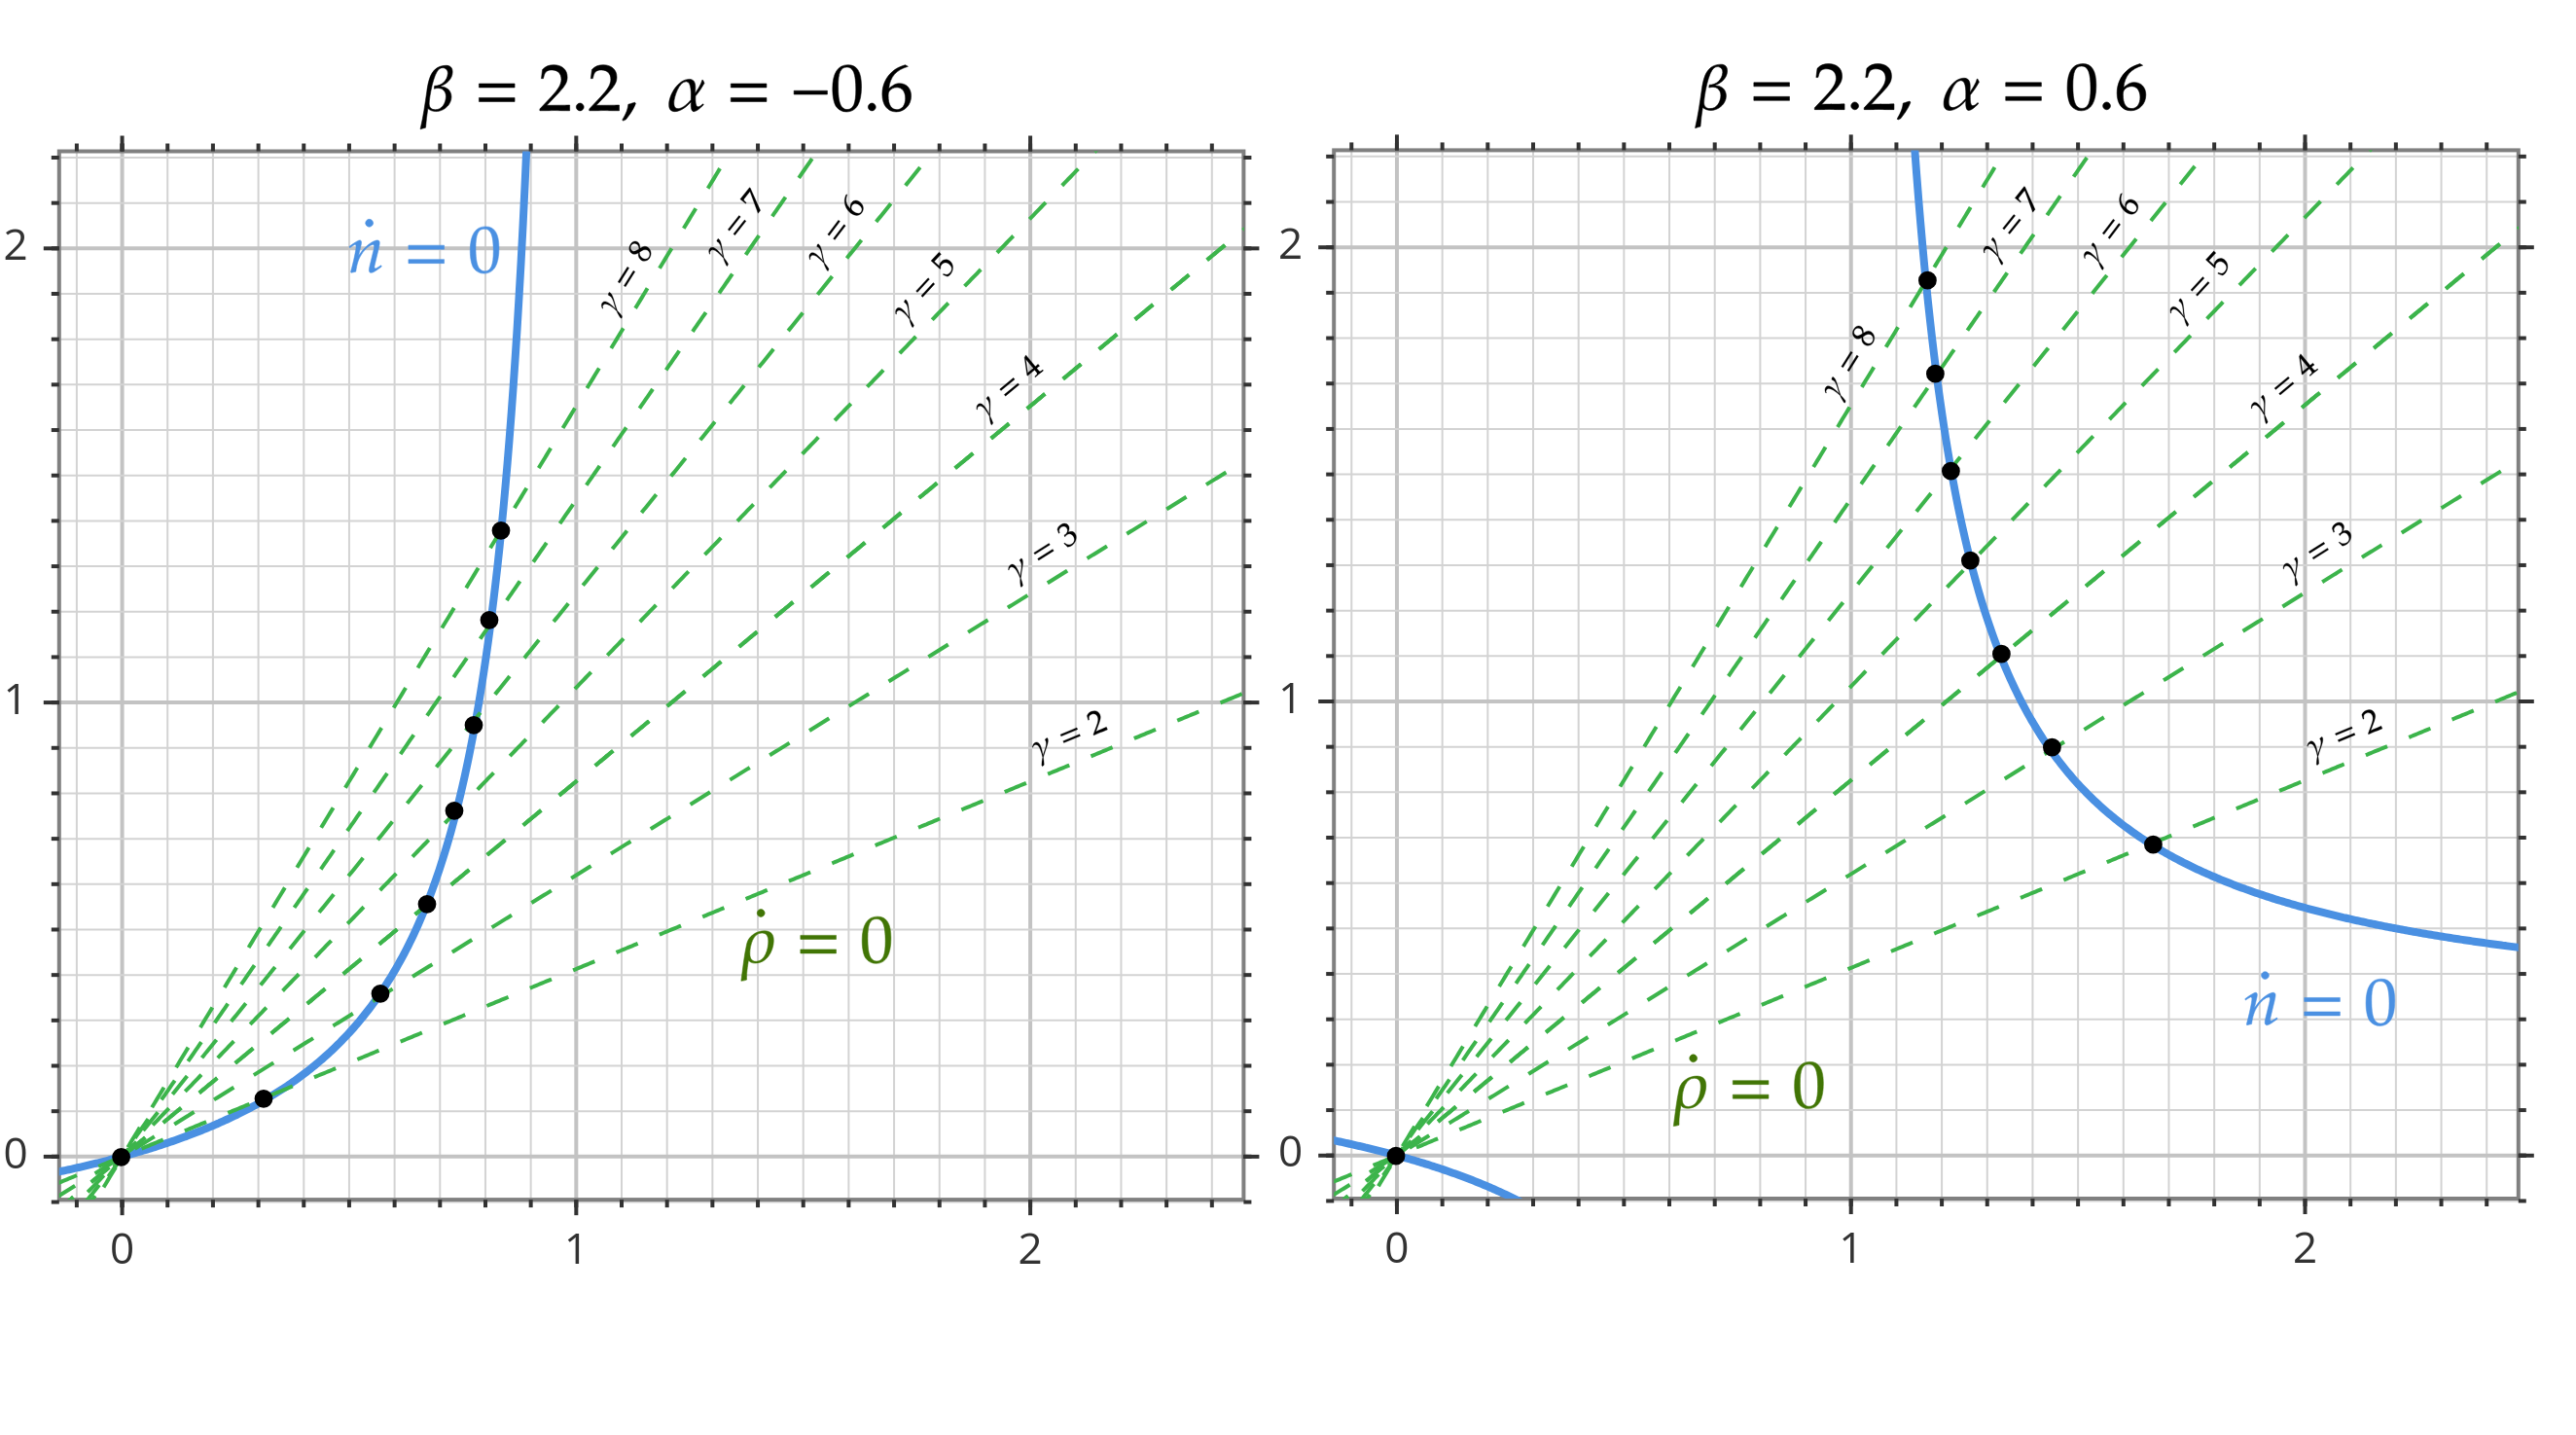
\includegraphics[width=\linewidth]{images/effectOfGamma.png} % first image
\end{figure}
\FloatBarrier

\subsubsection*{Effect of $\beta$}
Determining the effect of the parameter $\beta$ is not as straight forward as the other two parameters as it appears in both ODEs. However, we can plot the parameterized curve of $p^0_2(\beta)$ using (E.1.1) to see the effect of $\beta$ on the equilibrium point. The following figure summarizes the effect of $\beta$ on $p^0_2$.

\begin{figure}[h!]
	\centering
	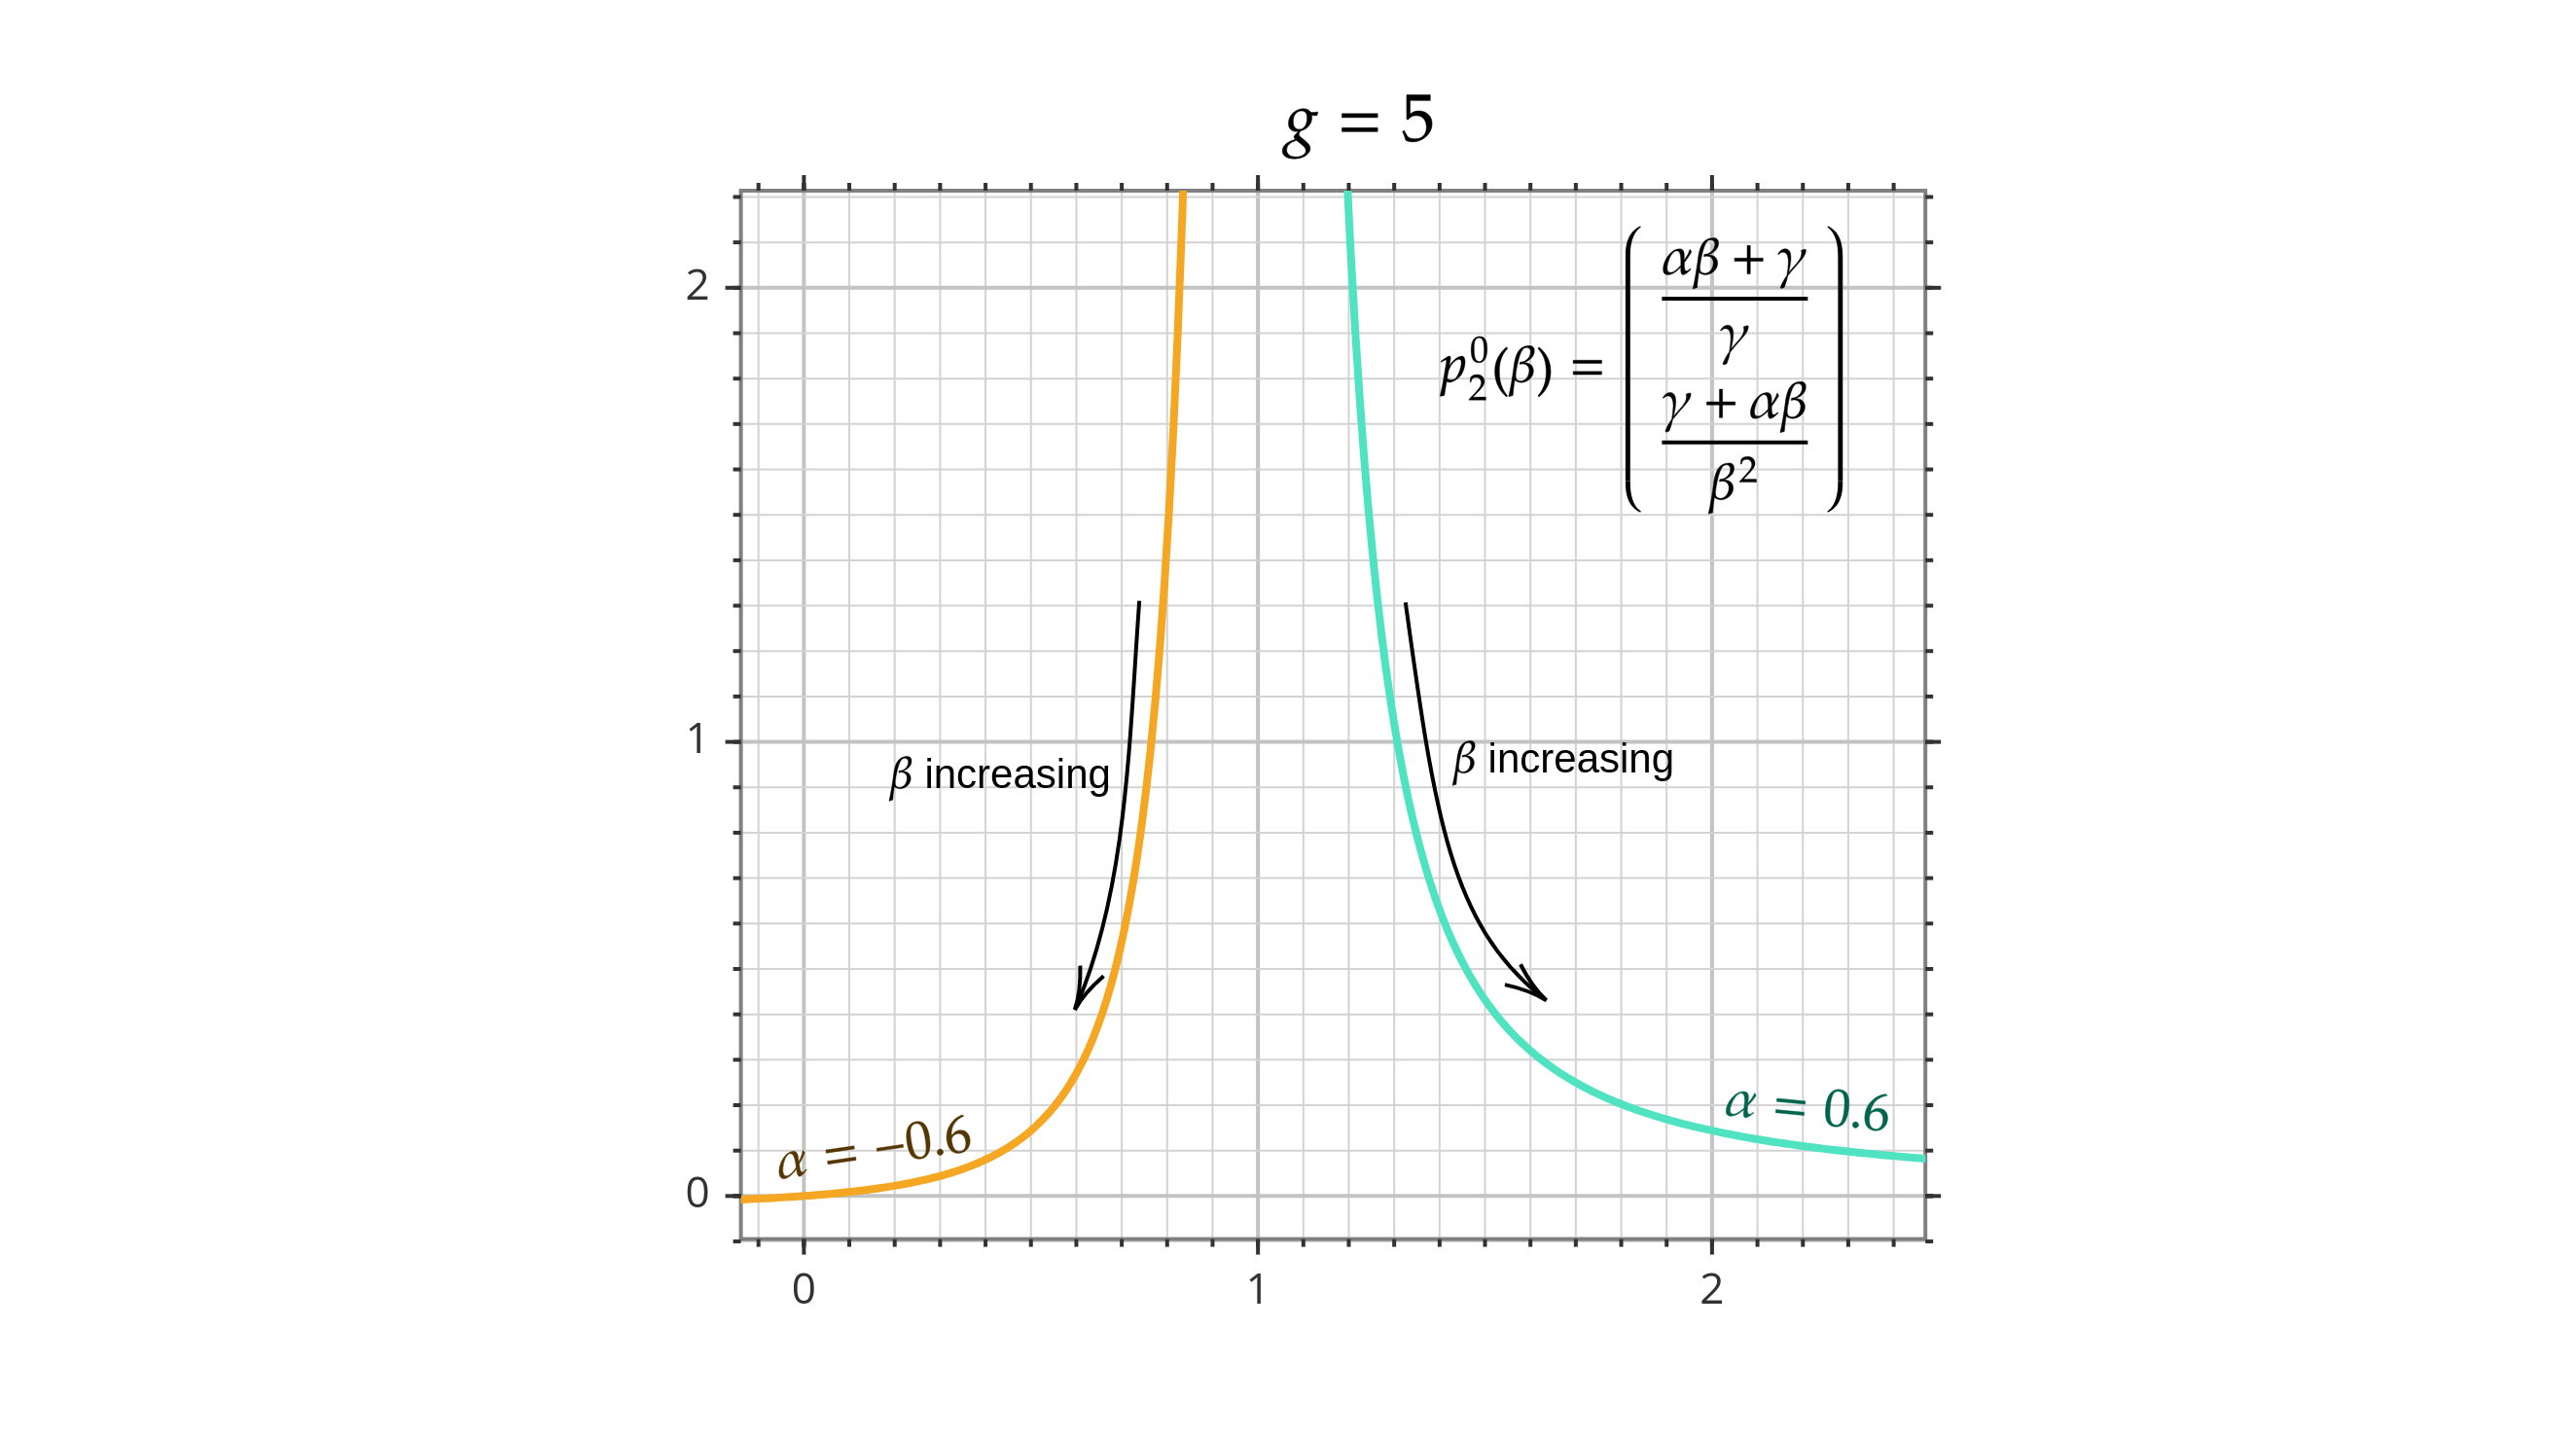
\includegraphics[width=\linewidth]{images/EffectOfBeta.png} % first image
\end{figure}
\FloatBarrier


\subsection*{Drug delivery}
In order to bring the drug-vessel interaction into play, we develop a ODE for $c(t)$ add approporite terms to the RHS of $\dot{n}$ and $\dot{\rho}$.
\[ \frac{dc}{dt} = \mu (\rho(t)f(t) - \sigma c(t)\rho(t)) - \boxed{\lambda c} \]
where $\mu$ has the unit [1/time], and $f(t)$ is the amount drug inside the capillary that has the unit [nmol per unit length]. Note that we have assumed the exchange of drug between the vessels and the region of interest is proportional to the difference in the concentration of drug in two different environments. Furthermore, the coefficient $\sigma$ has the units of [area/length] which is an indicator of the area coverage of the blood vessels. This parameter somehow characterizes the space filling and fractal structure of the blood vessels. This parameter should have some relations with the fractal dimension of a given vascular structure. Considering the dynamics of this parameter can possibly reflect some of the topological and non-local characterizations of the vascular network.



\subsubsection*{Basic and Simplified delivery scenario}
We assume that there is an infinite pool of drug (i.e. the patient is getting injected continuously) so the amount of drug per unit length in the capillary is constant $C_0$ [nmol per unit length].
\[ \frac{dc}{dt} = \mu \rho(t)(C_0 - \sigma c(t)).  \]

Also, note that we have ignored the radiation decay term to keep stuff simpler at this stage. The reason behind this choice is that at this stage, in adding the drug-vessel interaction, we will only consider a mass-action type interaction (i.e. chemical interactions), and no radio-biological interaction will be assumed (which has more complexity).

Another assumption that we make is that since the molecules of the drug are much smaller and simpler than the cells in the body, then we assume that they reach to equilibrium much more faster than the characteristic time scale of tip cell movement, and the death/generation of the cells. This basically means that we can simply assume $dc/dt=0$ to arrive at the following algebraic equation for $c$.
\[ C_0 = \sigma c(t). \]



\subsection*{Adding the drug-vessel interaction}
Presence of drug in the environment can have many different effects. It can kill/deactivate the existing tip cells (increasing $\delta_t$). Or it can change the rate at which the endothelial cells turn into the tip cells (changing the value of $\delta_b$). Or it can affect the tip cell division rate ($\lambda_s$). It can also affect the cellular migration of the tip cells and change the value of parameter $v$. The following lists the parameters corresponding to the amplitude of each of these interactions
\begin{itemize}
	\item $a_1$: changing the tip cell movement/migration
	\item $a_2$: killing/deactivating the tip cells
	\item $a_3$: changing the endothelial-to-tip cell conversion rate
	\item $a_4$: changing the tip cell division rate
\end{itemize}


\subsection*{Some discussions on drug interaction}
In mathematical modeling of biological processes, incorporating drug interactions can be complex, as the drug can influence various parameters of the system in different ways. The choice of interaction term often depends on the nature of the drug action and the available experimental data.
Here are a few common approaches to include drug interactions in the model:

\begin{enumerate}
	\item \textbf{Linear Interaction}: If the drug effect is proportional to its concentration, we can model the interaction linearly. For instance:
	\begin{align*}
		v(c) &= v_0 - a_1 c, \\
		\delta_v(c) &= \delta_{v0} + a_2 c,\\
		\lambda_b(c) &= \lambda_{b0} + a_3 c,\\
		\lambda_s(c) &= \lambda_{s0} - a_4 c.
	\end{align*}
	Here, \( v_0 \) and \( \delta_{v0} \) are the baseline motility and degradation rates without the drug, while \( a_1 \) and \( a_2 \) represent the sensitivity of these rates to the drug concentration. Similarly \( \lambda_{b0} \) and \( \lambda_{s0} \) are the baseline rates without the drug, and \( a_3 \), \( a_4 \) are the sensitivities of these rates to the drug concentration.

	
	\item \textbf{Hill Function}: If the drug effect exhibits saturation -- meaning it has a maximum effect regardless of concentration -- a Hill function can be appropriate:
	\begin{align*}
		v(c) &= v_0 \left(1 - \frac{a_1 c^h}{K_d^h + c^h}\right), \\
		\delta_v(c) &= \delta_{v0} \left(1 + \frac{a_2 c^h}{K_d^h + c^h}\right),\\
		\lambda_b(c) &= \lambda_{b0} \left(1 + \frac{a_3 c^h}{K_{d3}^h + c^h}\right),\\
		\lambda_s(c)& = \lambda_{s0} \left(1 - \frac{a_4 c^h}{K_{d4}^h + c^h}\right),
	\end{align*}
	Here, \( h \) is the Hill coefficient that determines the steepness of the response curve, and \( K_d \) is the drug concentration at which the effect is half of its maximum. With \( h \) as the Hill coefficient, and \( K_{d3} \), \( K_{d4} \) as the half-maximal effective concentrations for \( \lambda_b \) and \( \lambda_s \), respectively.
	
	\item \textbf{Michaelis-Menten Kinetics}: If the drug interaction is enzyme-like, you can model it using Michaelis-Menten kinetics:
	\begin{align*}
		v(c) &= v_0 \left(1 - \frac{a_1 c}{K_m + c}\right), \\
		\delta_v(c) &= \delta_{v0} \left(1 + \frac{a_2 c}{K_m + c}\right),\\
		\lambda_b(c) &= \lambda_{b0} \left(1 + \frac{a_3 c}{K_m + c}\right),\\	
		\lambda_s(c) &= \lambda_{s0} \left(1 - \frac{a_4 c}{K_m + c}\right),
	\end{align*}
	Where \( K_m \) is the Michaelis constant, representing the drug concentration at which the rate of reaction is half of its maximum. where \( K_m \) is the Michaelis constant, indicative of the concentration at which the reaction rate is half its maximum.
	
	\item \textbf{Exponential or Sigmoidal Functions}: For more complex drug effects, such as those that have a threshold effect or exhibit a sigmoidal dose-response, exponential or sigmoidal functions can be used.
\end{enumerate}

These interaction terms would be incorporated into the model by modifying the differential equations as follows:
\[
\frac{d\rho}{dt} = v(c)n - \delta_v(c) \rho,
\]

\[
\frac{dn}{dt} = (\lambda_s(c) - \delta_t) n + \lambda_b(c) \rho - \kappa n \rho,
\]

where \( \lambda_b(c) \) and \( \lambda_s(c) \) are now functions of the drug concentration that reflect the modulation of the endothelial-to-tip cell conversion rate and the tip cell division rate by the drug.

The form of the interaction should be chosen based on the biological mechanism of the drug action, the type and quality of experimental data available, and the ability to estimate the additional parameters introduced by these functional forms with the available data.
To decide which model to use, consider the following:

\begin{itemize}
	\item \textbf{Biological Mechanism}: Does the drug interact with its target in a manner that is competitive, non-competitive, or does it follow some form of cooperative binding? This will guide whether you use linear, Hill, or Michaelis-Menten kinetics.
	\item \textbf{Data Availability}: What kind of data do you have? If you have dose-response data, you can fit these models to the data to estimate parameters like \( a_1 \), \( a_2 \), \( h \), \( K_d \), or \( K_m \).
	\item \textbf{Parameter Estimation}: Can you estimate the additional parameters introduced by these functions? More complex models require more data for accurate parameter estimation.
\end{itemize}



\subsection{Simple Spatially Distributed 1D System}


In this section, we extend a simple ordinary differential equation (ODE) model for angiogenesis to include spatial dynamics. The original model captures the temporal evolution of the density of tip cells, the density of blood vessels, and the concentration of a drug delivered to a region. We now consider these variables as functions of both space and time, \(\rho(x,t)\), \(n(x,t)\), and \(c(x,t)\), to develop a partial differential equation (PDE) model that accounts for spatial growth and diffusion processes.

\subsubsection{Flux of Tip Cells}
A key concept in extending the model to incorporate spatial dynamics is the introduction of the flux of tip cells, denoted as \(J\). Flux is defined as the rate of flow of a property per unit area, which in this context is the flow of tip cells moving into a region. Mathematically, the flux \(J\) is given by the product of the density of tip cells \(n(x,t)\) and their velocity \(v\), i.e., \(J = nv\). This formulation allows us to quantify how the movement of tip cells contributes to the spatial development of blood vessels.

\subsubsection{Spatial Model Development}
We now proceed to develop the spatial model by modifying the equations from the original ODE model to incorporate spatial derivatives, reflecting the spatial dynamics of vessel formation, tip cell movement, and drug diffusion.


\subsubsection{Equation for Blood Vessel Density}
The blood vessel density \(\rho(x,t)\) is primarily affected by the extension of vascular structures due to the movement of tip cells and the degradation of these structures over time. Assuming homogeneous conditions without specific spatially-dependent growth mechanisms, the equation for \(\rho\) remains similar to the non-spatial model but now includes a spatial component:

\begin{equation}
	\boxed{\frac{\partial \rho}{\partial t} = vn - \delta_v \rho},
\end{equation}
where \(\delta_v\) represents the rate of vascular degradation.

\subsubsection{Equation for Tip Cell Density}
The spatial dynamics of tip cell density \(n(x,t)\) are influenced by their flux across the spatial domain. Incorporating the concept of flux, the balance equation for \(n\) in one dimension is given by:

\begin{equation}
	\boxed{\frac{\partial n}{\partial t} + \frac{\partial (nv)}{\partial x} = (\lambda_s - \delta_t) n + \lambda_b \rho - \kappa n \rho},
\end{equation}
where the terms on the right-hand side represent the generation and loss of tip cells, and the spatial derivative term accounts for their movement.

\subsubsection{Equation for Drug Concentration}
The drug concentration \(c(x,t)\) is affected by diffusion, permeation through the capillary walls, and any external sources of the drug. The equation accounting for these processes is:

\begin{equation}
	\frac{\partial c}{\partial t} = D\frac{\partial^2 c}{\partial x^2} - \mu c + f(x,t),
\end{equation}
where \(D\) is the diffusion coefficient, \(\mu\) represents the drug's permeability through capillaries, and \(f(x,t)\) is a source term for the drug.

\newpage

\section{Anderson Chaplain Model of Angiogenesis}

\subsection{Biological Facts and Basics}
\label{subsection:AndersonChaplainBiologyFacts}
The sequences of angiogenesis is assumed to be
\begin{enumerate}[(i),noitemsep]
	\item Tumor angiogenic factors (TAF) are secreted by the tumors under low oxygen stress. 
	\item Emergence of a chemical gradient of TAF between the tumor and the pre-existing vasculature.
	\item Endothelial cells lining the interior of the existing vasculature respond to this chemical clue by
	\begin{itemize}[noitemsep]
		\item Secreting digestive enzymes to loosen the basal lamina.
		\item Migrate from the disrupted membrane, up in the TAF gradient towards the tumor (i.e. chemotaxis). Look at the citations in the corresponding section)
		\item \label{item:InitialDistributionOfTipCells} The endothelial cells form into a few cell clusters \cite{Muthukkaruppan1982,Orme1996} which eventually become sprouts. Small, finger-like capillary sprouts are formed by accumulation of endothelial cells which are recruited from the parent vessel.
		\item The sprout grow in length and continue to move toward the tumor directed by the motion of the leading endothelial cells at the sprout tip.
	\end{itemize} 
	\item Further sprout extension occurs when some of the endothelial cells of the sprout wall begin to proliferate. Cell division is largely confined to a region just behind the cluster of mitotically inactive endothelial cells that constitute the sprout time. Note that \cite{Sholley1984} demonstrated that in the absence of endothelial cell proliferation, a restricted capillary network, which stops after a few days and never reaches the tumor, is formed. Thus, unless the endothelial cells undergo mitosis, the capillary sprouts cannot complete vascularization completely. \label{item:tipCeillsAreDividing}
	\item This process of sprout tip migration and proliferation of sprout-wall cells forms solid strands of endothelial cells amongst the extracellular matrix.
	\item The tip cells find their way through the extracellular matrix that consist of itersitial tissue, collagen fiber and fibronectin as well as other components.
	\item Interactions between the endothelial cells and the extracellular matrix, in particular fibronectin.
	\begin{itemize}
		\item \label{item:initialPhaseOfFibroNectin} \textbf{Initial distribution of fibronectin:} At the very early stages of angiogenesis, when the endothelial cells lining the parent vessels, are stimulated by TAF, they secrete enzymes to digest through the basal lamina of the parent vessel. This initial damage results in an increased vessel permeability \cite{Clark1981-pb}. This allows the plasma fibronectin from the blood to leak from the parent vessel and diffuse through the domain \cite{Hynes1989-je}. The diffusion coefficient of fibronectin has been measured to be $ 2\times10^{-7} \text{cm}^2\text{s}^{-1} $ \cite{Williams1982,Rocco1987}. This plasma fibronectin eventually binds to the extracellular matrix \cite{Oh1981,Deno1983,Clark1983}, thus prior to the start of angiogenesis we will have a gradient of fibronectin that is high near the parent vessel and gets lower away from the parent vessel. This has been experimentally observed by \cite{Paku1991} and \cite{Clark1982,Clark1981-pb,Clark1983}. It has also been experimentally observed that a higher concentration of laminin (another matrix macromolecule with similar adhesive properties to fibronectin) are initially found around the parent vessel \cite{Hynes1989-je,Paku1991}
		\item Cultured endothelial cells are known to synthesize and secrete cellular fibronectin (i.e. the insoluble form) \cite{Birdwell1978,Birdwell1980,1978,Macarak1978,Nerlich1991}. Note that the insoluble form is first secreted in the soluble form and then assembles into insoluble matrix.
		\item The expression of secreted fibronectin in cultured endothelial cells closely reflects the distribution of pre-existing fibronectin  observed in matrices \emph{in vivo} \cite{Vlodavsky1979,Hynes1989-je}
		\item The fibronectin secreted by the endothelial cells do not diffuse and bound the to extracellular matrix \cite{Birdwell1980,Hynes1989-je}.
		\item Fibronectin secreted by the endothelial cells is a major ligand between cells and matrix material in many situations.
		\item Endothelial cells use fibronectin for attachment to the matrix via integrins, a family of cell surface receptors \cite{Johansson1987,Hynes1989-je,Alberts2002a}.
	\end{itemize}
	\item Haptotaxis of the endothelial cells: migration of the endothelial cells up the gradient of adhesiveness \cite{Everitt1996,McCarthy1984,Carter1965}.
	\item Thus in addition to the chemotaxis of endothelial cells following the chemical gradient of TAF, there is a complementary haptotactic response to the fibronectin present within the extracellular matrix \cite{Bowersox1982}.
	\item Modes of the spatial growth:
	\begin{itemize}
		\item Initially, the sprouts arising from the parent vessel are essentially parallel to each other. 
		\item Tend to incline towards each other when the finger-like capillary sprouts have reached a certain distance from the parent vessel \cite{Paweletz1989} leading to numerous tip-to-tip and tip-to-sprout fusions known as anastomoses. This anastomoses leads to a network of poorly perfused loops and arcades.
		\item Form this process of anastomoses, the first signs of circulation can be recognized and from the primary loops, new buds and sprouts emerge repeating the angiogenic sequence of events.
		\item The process of emerging new capillary sprouts from the existing sprout tips is often called \emph{sprout branching}.
		\item As the sprouts approach the tumor, their branching dramatically increases until the tumor is eventually penetrated.
	\end{itemize}
	\item The repeated steps of angiogenesis: endothelial cell migration, sprout extension, cell proliferation and loop formation.
\end{enumerate}

\subsection{A Review of previous mathematical models}
\begin{itemize}
	\item Continuum and deterministic models for one dimension developed by \cite{Liotta1977,Balding1985,Chaplain1993,Byrne1995a,Orme1996}. These models were able to capture some features like average sprout density and network expansion rates. But was not able to capture more detailed information concerning the actual structure and morphology of the capillary network.
	\item More realistic 2D continuum models by \cite{Chaplain1995,Orme1997}: These models allowed a more detailed qualitative comparison with \emph{en vivo} observations about the spatial morphology of the networks. However, even these models were not able to capture the events like repeated sprout branching and hence overall dendrictic structure of the network.
	\item {\color{orange} Important: }More general continuum branching models \cite{Meinhardt1976,Meinhardt1982,Ermentrout1993}.
	\item Discrete probabilistic framework by \cite{Stokes1991} using stochastic differential equations. This model incorporated chemotaxis but not the Haptotaxis. Also, was not able to capture the fact that more branched appear as the network gets closer to the tumor. This effect is called the \textbf{brush border} effect\cite{Gimbrone1974,Ausprunk1977,Zawicki1981,Muthukkaruppan1982,Sholley1984}.
\end{itemize}



\textbf{Some notes about the fibronectin:} Fibronectin is a high molecular weight (about 500 kD) Glycoprotein (i.e. protein  + an Oligosaccharide) that binds to the membrane-spanning receptor protein called Integrin. On the other hand, they also bind to other extracellular matrix proteins like collage, fibrin, etc.

Fibronectin in blood plasma, is in soluble form (made in Liver), however, in the extracellular matrix, the Fibronectin is first secreted in soluble form (mostly by the fibroblast cells) and then assembles into an insoluble matrix in a complex cell mediated process. In the terminology above, the soluble fibronectin is called \emph{plasma fibronectin} and the insoluble form is called \emph{cellular fibronectin}.

\subsection{Details of the model}
Here in this section I will follow the model described in \cite{Anderson1998}. This model is based on the experimental data presented in \cite{Gimbrone1974} and \cite{Muthukkaruppan1982}. The variables of the model are as the following.

\begin{itemize}
	\item $ n = n(X,t): \Omega \times \R \to \R $: the endothelial-cell density (per unit area).
	\item $ c = c(X,t): \Omega \times \R \to \R $: the tumor angiogenic factor (TAF) concentration (nmol per unit area).
	\item $ f = f(X,t): \Omega \times R \to \R $: the fibronectin concentration (nmol per unit area).
	
\begin{strangeObs}[Ambiguity in the definition of one of the parameters]
	\label{strange:AmbiguityOfTipCell}
	As we read in \cite{Anderson1998}, $ n $ is introduced to be the ``endothelial-cell density''. However, I feel that it is not true and this variable should represent the ``endothelial \emph{tip} cell density''. I feel this way because it is the tip cells that are doing a random walk (thus diffusion) and reacting to the TAF and fibronectin gradients.
\end{strangeObs}
\end{itemize}

\subsubsection{Equations for endothelial cells}
The endothelial cells are moving in the space due to (1) their random motion (i.e. diffusion), (2) chemotaxis (moving up in the gradient of TAF), and (3) haptotaxis (moving up in the gradient of fibronectin). Combining these factors we will come up with the following flux for the tip cells
\[ J_n = -D_n \nabla n + \chi n \nabla c + \rho_0 n \nabla f. \]
where $ D_n $ is the diffusion coefficient of the endothelial cells, and $ \chi, \rho_0 $ are the sensitivity of chemotaxis and haptotaxis of endothelial cells due to the TAF and fibronectin gradients respectively.
Putting this in the continuoity equation, we will get

\[ \frac{\partial n}{\partial t} = -\nabla\cdot (-D_n \nabla n + \xi n \nabla c + \rho_0 n \nabla f) = D_n\nabla^2 n  - \nabla\cdot(\chi n\nabla c) - \nabla\cdot(\rho_0 n \nabla f).    \]


\begin{strangeObs}[Growth of the tip-cells are not considered in the model]
	As we discussed in \autoref{subsection:AndersonChaplainBiologyFacts} in \autoref{item:tipCeillsAreDividing}, the endothelial tip cells are dividing (otherwise the vascularization will not be completed). But in the PDE above, we didn't have any term for the tip cells proliferating or degrading.
\end{strangeObs}

\begin{strangeObs}[A problem with the diffusion coefficient of endothelial cells]
	As explained above, we are modeling the random mobility of endothelial tip cells by diffusion. However, according to the discussion (page 865 in \cite{Anderson1998}), it has been observed \cite{Rupnick1988} that when the migration of the endothelial cells are constrained by the surrounding cells, then their estimate for the for the diffusion coefficient the tip cells was too large and did not agree with experimental results. 
	
	Because of this observations, authors of \cite{Anderson1998} used a diffusion coefficient that was about 100 times smaller! (they cite to \cite{Bray2000} for this decision). I feel like this is not a good approach! The biological observation above is a signal that capturing the random mobility of the cell simply by diffusion is not a correct framework to use.
	
	Also, according to the discussion on page 886 of \cite{Anderson1998}), there are some in vivo experiments that indicate that there appear so the very little random mobility of endothelial cells at the capillary sprout tops \cite{Paweletz1989,Paku1991}.
\end{strangeObs}
In the PDE for tip cell density, the parameter $ \chi $ can depend on the concentration of TAF. We can model this interaction as (see the strange observation box below).

\[ \chi(c) = \chi_0 \frac{k_1}{k_1+c}. \] 

\begin{strangeObs}[The chemotaxis sensitivity seems not to be correct]
	In the model above by \cite{Anderson1998}, the authors are assuming that the functional form of $ \chi $ is given as
	\[ \chi(c) = \chi_0 \frac{k_1}{k_1+c}. \] 
	They say that the more realistic assumption is that the chemotactic sensitivity decreases with increased TAF concentration. They present the following references for this claim \cite{Lapidus1976,Lauffenburger1984,Sherratt1994,Woodward1995,Olsen1997}. This does not make sense for me. I feel like since the cell feels the chemicals by cell surface receptor binding, then the more chemicals available, the more strong is the signal for chemotaxis. So I feel that the appropriate model for this will be
	\[ \chi(c) = \chi_0\frac{c}{k_1 + c}. \]
\end{strangeObs}

\subsubsection{Equations for TAF}
To derive the equation for TAF concentration, first observe that TAF is secreted by the tumor cells where it starts diffusing into the space. I.e. the governing equation for TAF will be
\[ \frac{\partial c}{\partial t} = D_c\nabla^2 c - \theta c, \eqTag\label{eq:initialPDEForTAF} \]
where $ D_c $ is the TAF diffusion constant and $ \theta $ is the decay rate. We assume that during the initial stage of tumor secreting TAF, its distribution in the environment reaches a steady state which gives us the initial condition for the concentration of $ c $ in the domain.

In the stage that the angiogenesis begins (when we have an established steady state for $ c $), while the tip cells move up the gradient, TAF is used by uptake and binding to the cells \cite{Ausprunk1977,Hanahan1997}. This interaction can be modeled by
\[ \frac{\partial c}{\partial t} = -\lambda n c, \]
where $ \lambda $ is a constant.

\begin{strangeObs}[TAF interaction with cells does not seem to be correct]
	In the model above (from \cite{Anderson1998}), the uptake and binding of TAF to the tip cells is modeled in a mass action kinetic way. I have a feeling that this might not be true and it should be modeled by Michaelis-Menten equation. Also, this model assumes that the used TAF is not get replaced, but I feel that as long as tumor is under oxygen stress, the secreting mechanism of TAF in tumor will still be active. 
\end{strangeObs}


\begin{beCareful}[To much intuition is not good]
	The way that the model above is presented is not appealing for me at all. This is the way that \cite{Anderson1998} does, and I think there are more than enough common sense floating around! For instance, they say that in the initial stage, the tumor secretes the TAF and it starts diffusing in the environment while degrading and eventually reaches steady state (which is fair up to now). Then, they say that during the angiogenesis stage the differential equation governing the concentration of TAF is different (Which also makes sense). My problem is that I want to see both of the terms in a single PDE and then by appropriate mathematical treatment (slow-fast dynamics, perturbation theory, etc) arrive at the conclusions that they stated using the commons sense. I need to do this for my thesis.
\end{beCareful}

\subsubsection{Equations for fibronectin}
As we discussed in the biology background subsection, the endothelial tip cells tend to move up in the gradient of fibronectin. Fibronectin is present in the domain before angiogenesis. As the tip cells do haptotaxis (moving up {\color{red} (up or down?)} in the gradient of fibronectin) they use some fibronectin to connect to the ECM. Tip cells also secrete fibronectin which dose not diffuse. Thus the corresponding differential equation will be 
\[ \frac{\partial f}{\partial t} = \omega n - \mu n f, \]
where $ \omega $ is the production rate of $ f $ by the tip cells and $ \mu $ is the rate at which the tip cells use fibronectin to bind to the ECM.

\begin{strangeObs}[The model for fibronectin dynamics is too simple]
	The model above for the time evolution of fibronectin is given by \cite{Anderson1998}. According to our detailed discussion in \autoref{item:initialPhaseOfFibroNectin}, I feel like this model is too simple to capture the time evolution of the fibronectin. We are assuming that the fibronectin is used and produced only by the tip cells (if by \autoref{strange:AmbiguityOfTipCell} we come to the conclusion that $ n $ represents the tip cells). This implies that the stalk cells are not producing fibronectin which might not be true. Also, as assume that as soon as the process of angiogenesis starts, the leakage of fibronectin from the parent vessel into the domain stops. According to the parameters in \autoref{tab:AndersonChaplainModelRealisticParameters}, the time scale happens to be $ \tau = L^2/D_c \approx 2\ \text{days}  $. Since in \autoref{item:initialPhaseOfFibroNectin} we discussed that the reason of the initial distribution of fibronectin is the damage to the basal lamina of the parent vessels, then I feel like in the span of several days that dame might still persist so we might still have the leakage of fibronectin to the domain.
\end{strangeObs}

\begin{strangeObs}[The initial condition for fibronectin is too intuitive]
	\label{strange:FibronectinInitialConcentration}
	As we will see in {\color{red} [add the cross reference for the fibronectin initial condition here]}, the initial condition for fibronectin concentration, although makes sense, but it is not appropriately modeled compared to what we did for TAF (see Equation (\autoref{eq:initialPDEForTAF}))
\end{strangeObs}

\begin{summary}
	The complete set of equations will be give as
	\begin{align*}
		&\frac{\partial n}{\partial t} =  D_n\nabla^2 n  - \nabla\cdot(\chi n\nabla c) - \nabla\cdot(\rho n \nabla f), \\
		&\frac{\partial c}{\partial t} = -\lambda n c, \\
		&\frac{\partial f}{\partial t} = \omega n - \mu n f,
	\end{align*}
\end{summary}
\begin{remark}
	We assume that non of species, i.e. tip cells, TAF and fibronectin leave the domain of simulation. Thus the boundary condition is give as 
	\[ \hat{\xi} \cdot J_n = 0. \]
\end{remark}

\subsection{Non dimensionalization of the system}
For an easier analysis of the system we first need to write the system in non dimensionalized way. Consider the following change of variables
\begin{align*}
	& n = N_0 \tilde{n}, && c = C_0 \tilde{c}, &&& f = F_0\tilde{f}, \\
	& t = \underbrace{\tau}_{\tau = L^2/D_c} \tilde{t}, && x = L \tilde{x}.
\end{align*}
Substituting these change of variables in the model we will get the following non dimensionalized form of the model. Note that we remove the tilde symbol for more clear look.
\begin{align*}
	&\frac{\partial n}{\partial t} = D \nabla^2 n - \nabla\cdot(\frac{\chi}{1+\alpha c} n\nabla c) - \nabla\cdot(\rho n \nabla f), \\
	&\frac{\partial c}{\partial t} = -\eta n c, \\
	&\frac{\partial f}{\partial t} = \beta n - \gamma n f,
\end{align*}
where 
\begin{align*}
	& D = \frac{D_n}{D_c}, && \chi = \frac{C_0\chi_0}{D_c},\ \alpha = \frac{C_0}{k_1} && \rho = \frac{f_0\rho_0}{D_c},\\
	& \eta = \frac{L^2\lambda N_0}{D_c}, && \beta = \frac{L^2\omega N_0}{F_0 D_c}, && \gamma = \frac{L^2\mu N_0}{D_c}.
\end{align*}

\subsection{Some discussions on the parameters used}
The following table summarizes the realistic values for the model parameters discussed in \cite{Anderson1998}.

% Please add the following required packages to your document preamble:
% \usepackage[table,xcdraw]{xcolor}
% Beamer presentation requires \usepackage{colortbl} instead of \usepackage[table,xcdraw]{xcolor}
% Please add the following required packages to your document preamble:
% \usepackage[table,xcdraw]{xcolor}
% Beamer presentation requires \usepackage{colortbl} instead of \usepackage[table,xcdraw]{xcolor}
% Please add the following required packages to your document preamble:
% \usepackage[table,xcdraw]{xcolor}
% Beamer presentation requires \usepackage{colortbl} instead of \usepackage[table,xcdraw]{xcolor}
\begin{table}[!ht]
	\centering
	\begin{tabular}{|c|c|c|}
		\hline
		\textbf{Parameter}       & \textbf{Value {[}units{]}}                       & \textbf{Reference} \\ \hline
		$D_n$                    & $10^{-10}\ [\text{cm}^2\text{s}^{-1}]$           &  \cite{Bray2000}   \\ \hline
		$ D_c $                  & $2.9 \times 10^{-7}\ [\text{cm}^2\text{s}^{-1}]$  & \cite{Bray2000,Sherratt1990} \\ \hline
		$\chi_0$                 & $ 2600\ [\text{cm}^2\text{s}^{-1}\text{M}^{-1}] $ &  \cite{Stokes1990}  \\ \hline
		$ \rho_0 $               & same as $\chi_0$ but $ \chi_0  > \rho_0 $        & \cite{Anderson1998}   \\ \hline
		$ c_0 $                  & $10^{-10}\ [M]$                               &   \cite{Stokes1990} \\ \hline
		$ f_0 $                  & $10^{-10}\ [M]$                               &  \cite{Terranova1985}  \\ \hline
		$ \lambda, \omega, \mu $ & no available estimates.                          &  \cite{Hynes1989-je}  \\ \hline
		$ L $                    &   $ 2\ [mm] $       &     \cite{Gimbrone1974}     \\ \hline
	\end{tabular}
	\caption{The biologically realistic parameter values for the Anderson-Chaplain model.}
	\label{tab:AndersonChaplainModelRealisticParameters}
\end{table}
\FloatBarrier


\subsection{Simulating the model}

\subsection{Simulation Domain}
to be expanded: square $ [0,1]\times [0,1] $. With the tumor located at $\set{1} \times [0,1] $ and the parent vessel located at $ \set{0} \times [0,1] $.

\subsubsection{Initial condition for tip cell density}
As we discussed in \autoref{item:InitialDistributionOfTipCells} the tip cells, after getting stimulated by TAF form small clusters. Thus we assume that the initial concentration of the tip cells are give as
\[ n(x,y,0) = e^{-x^2/\xi_3} \sin^2(3\pi y). \]
\begin{figure}[!ht]
	\centering
	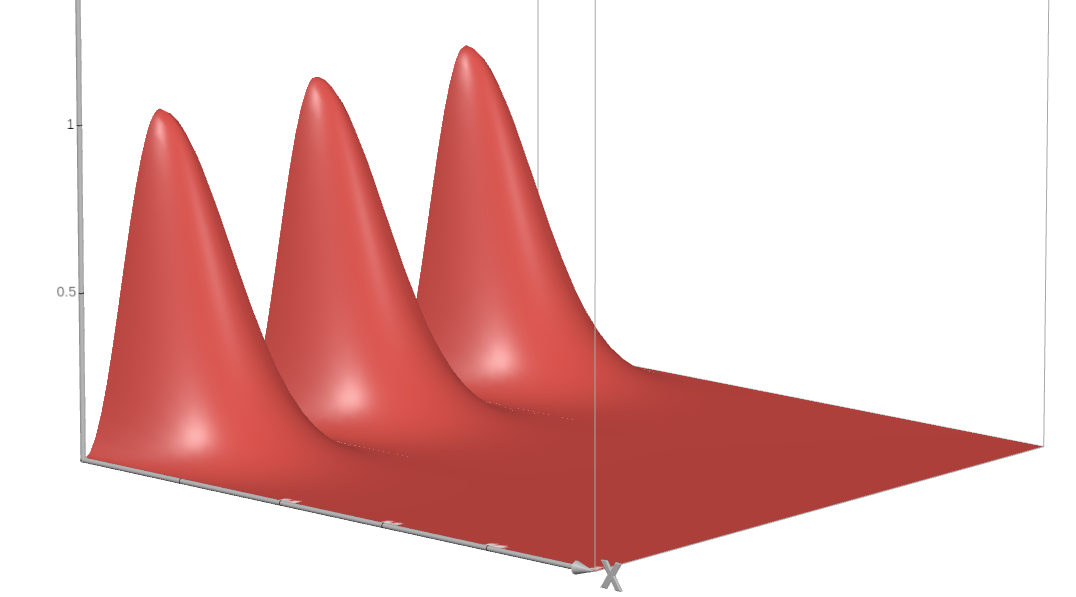
\includegraphics[width=0.4\linewidth]{images/tipCellInitialDensity}
	\caption{Tip cell initial density.}
	\label{fig:tipcellinitialdensity}
\end{figure}


\subsubsection{Initial condition for TAF}
Assuming Equation \autoref{eq:initialPDEForTAF} models the initial phase of the time evolution of TAF, then we can assume that the steady state of that equation is the initial condition for the phase that the angiogenesis starts happening. Depending on the initial configuration of the tumor in the domain, \cite{Anderson1998} came up with two biologically interesting initial condition. 

\textbf{Case 1: A column of tumor cells or larger circular implant.} For this case the initial concentration of TAF will be
\[ c(x,y,0) = e^{-(1-x)^2/\xi_1}, \qquad (x,y) \in [0,1] \times [0,1]. \]

\textbf{Case 2: A small circular tumor centered at (1,1/2)}. In this case the initial concentration of TAF is given by (\cite{Anderson1998} and they reference \cite{Chaplain1995,Chaplain1996} for the equation)
\[ c(x,y,0) = \begin{cases}
	1, &\qquad 0\leq r\leq r_0, \\
	\frac{(\nu - r)^2}{\nu - r_0}, &\qquad r_0 \leq r \leq 1,
\end{cases} \]
where $ \nu $ is a positive constant and $ r $ is given by
\[ r = \sqrt{(x-1)^{2} + (y-1/2)^2}, \]
assuming that the tumor is centered at $ (1,1/2) $ with a radius of $ r_0 $. Note that $ \nu $ is in fact showing the concentration right at the edge of the tumor. To make the transition between concentration $ c $ inside the tumor (i.e. $ 0 \leq r \leq r_0 $) and outside the tumor (i.e. $ r_0 \leq r \leq 1 $) continuous, the value of $ \nu $ should be $ \boxed{\nu = r_0 + 1} $. We can see this by simply trying to force the function $ c(x,y,0) $ to be continuous. The following figure illustrates the initial concentration of TAF for $ r_0 = 0.2 $ (thus $ \nu = 1.2 $).
\begin{figure}[!ht]
	\centering
	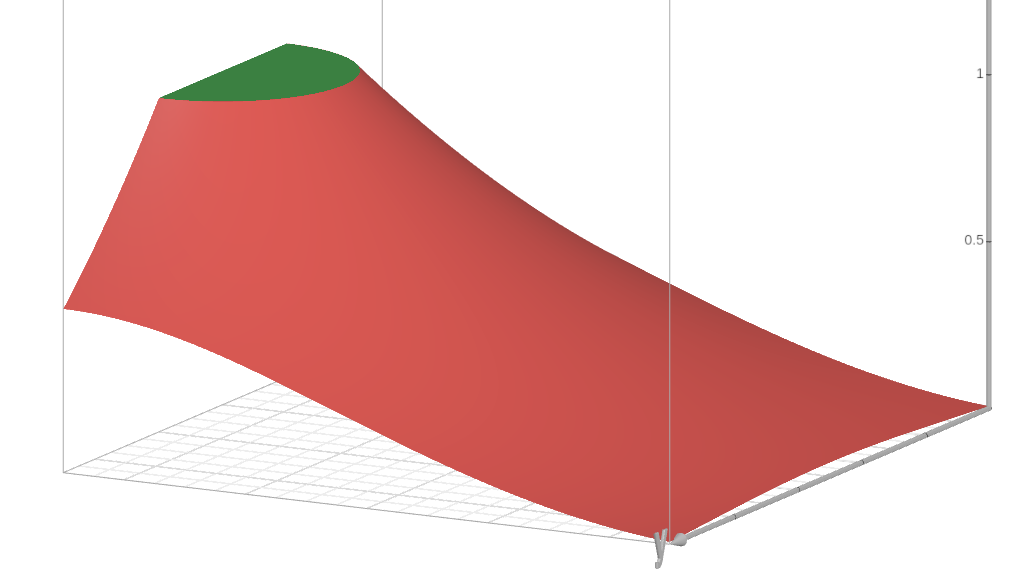
\includegraphics[width=0.5\linewidth]{images/TAFInitialConcentrationSmallTumor}
	\caption{Initial concentration of TAF for small tumor with radius $ r_0 = 0.2 $ centered at $ (1,1/2) $. The green region shows the tumor inside which the concentration of TAF is assumed to be 1.}
	\label{fig:initialConcentrationOfTAFSmallTumor}
\end{figure}


\begin{beCareful}[I am not sure if the formulas above are really the steady state solution of TAF PDE]
	Note that the initial concentration of TAF should be the steady state of Equation \autoref{eq:initialPDEForTAF}. \cite{Anderson1998} claims that the two cases above are the steady state solutions for the early stage TAF PDE. I have not checked this yet and I need to evaluate if this is really true.
\end{beCareful}


\subsubsection{Initial condition for Fibronectin}
The initial condition for fibronectin has been a more phenomenological one in \cite{Anderson1998}. They Assumed the initial concentration of fibronectin is given by
\[ f(x,y,0) = k e^{-x^2/\xi_2}, \qquad (x,y) \in [0,1] \times [0,1], \] 
where $ 0<k<1 $ and $ \xi_2 > 0 $. As discussed in \autoref{item:initialPhaseOfFibroNectin} this choice of initial conditions is justified up to some degree. However look at \autoref{strange:FibronectinInitialConcentration} for a discussion about possible alternative approaches to find a more realistic initial condition.



\subsection{Make it a Combo! Adding Stochastic Model to Generate Vascular Networks}

\subsection{Some Thoughts}
\subsubsection{Discrete vs. continuous model}
For me, the distinction between discrete model and the continuous model discussed above is just the difference between solving a SDE (which will give us some trajectories) vs. solving the corresponding Fokker-Plank equation. However observe that, in SDE trajectories, we can measure some quantities like the number of branches, number of loops, the tortuosity, distribution of the length segments, etc. On the other hand, the corresponding Fokker-Plank equation (the advection-diffusion PDE) gives us the time evolution of the tip cell density. So the following is my question

\begin{openQuestion}
	Given an SDE, is it possible to write down a differential equation (like the Fokker-Plank equation) that can capture a measurement of interest? Like the time evolution of the average number of collisions between $ n $ trajectories of the SDE.
\end{openQuestion}
Here are some possible steps to find the answer to the question above.
\begin{observation}[Steps to solve the question above]
	The overall theme of solving the question above is to generalize the Fokker-Plank equation of an SDE such that we can write down a similar PDE for any measurement of interest. 
	\begin{enumerate}[(I)]
		\item First, try to think about the Fokker-Plank equation in this framework. I.e. try to observe what kind of measurement is the variable $ \rho $ whose time evolution is captured by the Fokker-Plank equation.
		\item Try to abstract the notion of $ \rho $. I.e. What are the properties of $ \rho $ that help in developing the Fokker-Plank equation?
	\end{enumerate}
\end{observation}


\subsection{Important citations of this paper}
\begin{itemize}[noitemsep]
	\item biology of the angiogenesis
	\begin{itemize}[noitemsep]
		\item Embryo angiogenesis \cite{Graham1992}.
		\item Angiogenesis in tissue repair \cite{Arnold1991,Pettet1996}.
		\item Uncontrolled angiogenesis in tumors, arthritis, abnormal neovascularization of the eye, duodenal ulcers, and following myocardial infarction \cite{Folkman1985,Folkman1995,Folkman1987}.
		\item Pathological examples of angiogenesis \cite{Muthukkaruppan1982,Ribatti2008}.
	\end{itemize}
	\item Angiogenic factors:
	\begin{itemize}
		\item Several angiogenic factors like vascular endothelial growth factor (VEGF), acidic and basic fibroblast growth factor (aFGF, bFGF), angiogenin, etc has been isolated \cite{Folkman1987,Relf1997}.
		\item Endothelial cell receptors for these angiogenic factors \cite{Millauer1993,Hatva1995,Mandriota1995,Fong1995,Hewett1996,Patterson1996,Kappel1999,0deab5d12daa4d32b398e5c5f589f651,Hanahan1997}
		\item Effect of disrupting the angiogenic factors on the final structure of the capillary network \cite{Dumont1994,Fong1995,Sato1995,Hanahan1997}.
	\end{itemize}
	\item Initial response of the endothelial cells to the angiogenic factors is a chemotatic one \cite{Sholley1984,Terranova1985,Paweletz1989,Stokes1990}.
	\item New finger-like capillary sprout formation \cite{Cliff1963,Warren1966,Ausprunk1977,Sholley1984}
	\item New tip cells finding their way through the extracellular matrix \cite{Liotta1983,Paweletz1989}.
\end{itemize}


\newpage
\section{Idea Bin!}
This section might have very simple, basic and sometimes silly ideas that came into my mind during developing some models and I thought they might worth trying
\begin{itemize}
	\item Developing a model for a weighted graph generation. I suspect a weighted graph might have all the necessary information we want.
\end{itemize}

